V rámci této kapitoly se pokusím co možná nejkomplexněji srovnat hybridní a nativní přístup. Jejich porovnání se bude týkat tří klíčových oblastí z životního cyklu aplikace.

\section{Způsob vývoje}
\subsection{Náročnost vývoje}
\subsubsection{Lidské zdroje a finance}
Tyto dvě kritéria jsem spojil do jednoho, protože spolu velmi úzce souvisí. Cena vývoje aplikace totiž naprosto dominantně záleží na lidech, kteří jí vytváří. Je zřejmé, že výsledná cena závisí na mnoha faktorech, jako je například typ aplikace (jiné náklady bude třeba vynaložit na tvorbu jednoduché To-Do aplikace, jiné na vývoj 3D hry), počet platforem, na které budeme aplikaci portovat nebo aktuální situace na trhu.

Obecně se však uvádí, že vývoj hybridní aplikace je oproti nativní variantě levnější. Hlavním důvodem je, že vývojáři znalý webových technologií stojí méně než kvalifikovaní vývojáři znalí technologií nutných pro vývoj pro konkrétní platformu. Odhaduje se, že vývoj nativní aplikace stojí mezi 20 000 a 150 000 dolary \cite{mrc_native_wrong_choice}.

V obecné rovině také platí, že weboví vývojáři jsou na pracovním trhu poměrně lehce k sehnání a řada firem již takové vývojáře dokonce zaměstnává interně. V takovém případě je využití hybridního přístupu obzvláště lákavé.

Dle trendů na pracovním trhu, které sleduje server indeed.com, je poptávka po vývojářích ovládajících technologii HTML 5 skutečně velká. Jedná se dokonce o nejvíce vyžadovanou dovednost ze všech pracovních nabídek, které server pravidelně analyzuje. Strmý růst poptávky po HTML 5 vývojářích vidíme na grafu \ref{fig:HTML5Jobs}.

\begin{figure}\centering
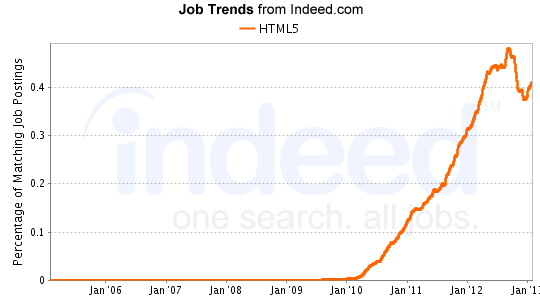
\includegraphics[width=1.0\textwidth]{jobgraph_html5.png}
\caption{Vývoj nabídek zaměstnání pro HTML5 vývojáře \cite{job_indeed}}
\label{fig:HTML5Jobs}
\end{figure}

S tímto trendem se logicky svezla i poptávka po vývojářích specializovaných na přední hybridní framework PhoneGap.

\begin{figure}\centering
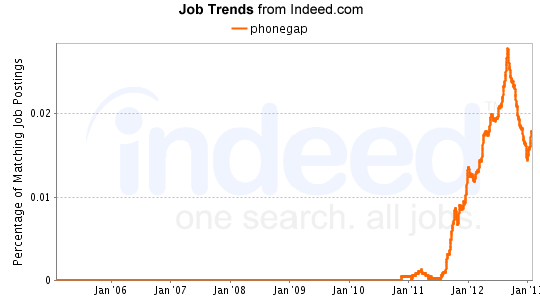
\includegraphics[width=1.0\textwidth]{jobgraph_phonegap.png}
\caption{Vývoj nabídek zaměstnání pro PhoneGap vývojáře \cite{job_indeed}}
\label{fig:PhoneGapJobs}
\end{figure}

Zajímavým ukazatelem je také průměrná mzda, kterou vývojáři s těmito schopnostmi dostávají. Průměrná mzda na pozicích, kde je vyžadována znalost HTML5 je 84 000 amerických dolarů ročně \cite{job_indeed}. Zaměstnanec na pozici „HTML Developer“ pak pobírá 75 000 dolarů za rok \cite{job_indeed}. Velice blízko těmto číslům je i průměrná mzda na pozicích, kde je jako schopnost vyžadována znalost frameworku PhoneGap, která dosahuje výše 86 000 dolarů \cite{job_indeed}.

Pokud se podíváme na nativní vývojáře, tak zjistíme, že poptávka po nich je jen nepatrně nižší.

\begin{figure}\centering
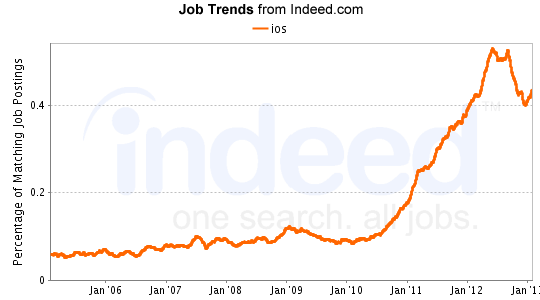
\includegraphics[width=1.0\textwidth]{jobgraph_ios.png}
\caption{Vývoj nabídek zaměstnání pro iOS vývojáře \cite{job_indeed}}
\label{fig:iOSJobs}
\end{figure}

Na datech o průměrné mzdě, která je nabízena vývojářům ovládajícím technologie pro vývoj pro iOS, je vidět, že jsou vývojáři s těmito schopnostmi nákladnější. Průměrná mzda v této oblasti dosahuje výše 89 000 dolarů za rok. Zaměstnanec na pozici „iOS Mobile Developer“ pobírá ročně 104 000 dolarů. O něco levnější je cena práce vývojáře pro platformu Android, kde si „Android Developer“ přijde na 101 000 dolarů za rok.

Dalším faktorem je také výše zmíněný počet platforem, pro které bude aplikace vyvíjena. Zatímco v případě vývoje pro jedinou platformu nemusí být rozdíl v nákladech na vývojáře markantní, v případě cílení na dvě nebo více platforem již náklady na nativní vývojáře strmě rostou. Tuto situaci názorně dokládá následující tabulka, která ukazuje odhadované náklady na vývoj multiplatformní aplikace (iOS, Android, Windows Phone) pomocí nativní i hybridní cesty.

\begin{table}\centering
	\caption[Srovnání ceny hybridního a nativního přístupu při vývoji aplikace pro 3 platformy]{Srovnání ceny hybridního a nativního přístupu při vývoji aplikace pro 3 platformy \cite{globant_hybrid}} 
	\label{tab:ComparsionCost}
		\begin{tabular}{|c|c|c|c|}\hline
			Profese	& Počet & Hodin [rok] & Roční náklady [USD]
			\tabularnewline \hline \hline
					iOS Architekt	& 1 & 2 000 & \$200 000
			\tabularnewline \hline
					iOS Developer	& 3 & 6 000 & \$300 000
			\tabularnewline \hline
				\textbf{Celkem}	& \textbf{4} & \textbf{8 000} & \textbf{\$500 000}
			\tabularnewline \hline \hline
				JavaScript Architekt	& 1 & 2 000 & \$200 000
			\tabularnewline \hline
				JavaScript Developer	& 3 & 6 000 & \$300 000
			\tabularnewline \hline
				iOS Developer	& 1 & 2 000 & \$100 000
			\tabularnewline \hline
				Android Developer	& 1 & 2 000 & \$100 000
			\tabularnewline \hline
				Windows Phone Developer	& 1 & 2 000 & \$100 000
			\tabularnewline \hline
				\textbf{Celkem}	& \textbf{7} & \textbf{14 000} & \textbf{\$800 000}
			\tabularnewline \hline \hline
				\textbf{Při vývoji pro 3 platformy} & & &
			\tabularnewline \hline
				Nativní tým & 12 & 24 000 & \$1 500 000
			\tabularnewline \hline
				Hybridní tým & 7 & 14 000 & \$800 000
			\tabularnewline \hline
				\textbf{Úspory}	& \textbf{42 \%} & \textbf{42 \%} & \textbf{47 \%}
			\tabularnewline \hline
		\end{tabular}
\end{table}

\subsubsection{Složitost}
Jednoznačně určit, který přístup je pro vývojáře složitější, je náročné. Pro každého jedince je subjektivně složité něco jiného.

Obecně lze říci, že vývoj nativních aplikací vyžaduje rozsáhlejší znalosti, než-li je tomu při vývoji pomocí webových technologií. I hybridní vývojář však musí velmi dobře rozumět javascriptovému frameworku, který používá. Je třeba si uvědomit, že vývoj mobilních aplikací se v mnoha ohledech výrazně liší od vývoje klasických webových stránek.

\subsection{Rychlost vývoje}
Toto kritérium je více než všechny ostatní závislé na komplexnosti vyvíjené aplikace. Velmi jednoduchá aplikace může být vyvinuta v řádu dnů až týdnů jak nativně tak hybridně. U složitější aplikace zas doba strávená jejím vývojem závisí na jiných faktorech (počet vývojářů, počet platforem apod.). Výzkum společnosti Forrester Research udává, že vývoj nativní aplikace zabere vývojovému týmu průměrně 6 měsíců \cite{mrc_native_wrong_choice}. Pokud je aplikace vyvíjena pro více platforem, je jasné, že se doba vývoje prodlouží kvůli neustálé nutnosti koordinace vývojových týmů s cílem přinést konzistentní UX[c] napříč platformami.

Zřejmě tedy nebudeme daleko od pravdy, když řekneme, že v obecném slova smyslu je vývoj hybridních aplikací méně časově náročný než vývoj nativní. To je způsobeno zejména možností využití jedné sady zdrojových kódů pro port aplikace na různé platformy.

\subsection{Nástroje}
\subsubsection{Vývojové prostředí}
Volba správného vývojového prostředí je pro pohodlný a rychlý vývoj mobilní aplikace klíčová. Vývojáři nativních aplikací v drtivé většině používají vývojová prostředí dodávaná s SDK konkrétní platformy. Pro iOS tedy vyvíjejí v XCode, pro Android v Eclipse, pro Windows Phone ve Visual Studiu a tak podobně. Tato prostředí jim poskytují možnost správy projektů, tvorby zdrojového kódu a také nezbytné ladící nástroje. Pomocí těchto prostředí je rovněž možné odeslat hotovou aplikaci na oficiální tržiště dané platformy.

Vývojáři hybridních aplikací mají ve volbě svého vývojového prostředí zdánlivě větší svobodu. Od uvedení nástroje PhoneGap Build (viz. kapitola \ref{Sec:PhoneGapBuild}) již nejsou nuceni pro vytvoření nativních instalačních balíčků používat SDK konkrétní platformy. V zásadě nic pak vývojáři nebrání používat pro vývoj libovolné vývojové prostředí dle vlastních preferencí (například oblíbený textový editor).

\subsubsection{Testování a debugging}
V tomto případě je situace podobná jako u vývojových prostředí. Pro nativní vývojáře jsou ladící a testovací nástroje dodávány jako součást SDK. Přímo z vývojového prostředí tedy spouští svou aplikaci v emulátoru a využívají debugovací nástroje vytvořené přímo za účelem ladění mobilních aplikací pro danou platformu.

Hybridní vývojáři mají situaci obtížnější. Mohou sice také využívat nativních nástrojů z SDK, ale pouze v omezené míře, neboť tyto nejsou vhodné pro ladění aplikací napsaných webovými jazyky. Hybridní vývojáři proto nejčastěji používají kombinaci nástrojů (nativní emulátor + webový prohlížeč + Ripple + Weinre) [viz kapitola \ref{Sec:DebugaTest}]. Nativní emulátor mohou spouštět buď z vývojového prostředí určeného pro vývoj nativních aplikací (například Eclipse) nebo pomocí konsolového interface, který poskytuje například framework PhoneGap.

\subsubsection{Podpora}
Každý vývojář se v průběhu vývoje mnohokrát dostane do situace, kdy neví jak dál a potřebuje pomoci. Tuto pomoc může získat z celé řady zdrojů jako jsou například knižní příručky, placená podpora, internetové články a internetová komunitní fóra.

V této oblasti mají nativní vývojáři zatím jasně navrch, což je dáno zejména tím, že hybridní přístup je poměrně nový. Počet knih i internetových příruček zabývajících se hybridním vývojem je oproti nativnímu signifikantně nižší. Kolem vývoje nativních aplikací pro konkrétní platformu je vytvořen celý prstenec nástrojů, které mohou vývojáři používat, když potřebují pomoci. Jedná se o IRC chaty, specializované diskuzní skupiny či možnost nechat si poradit od odborníků v rámci office hours (Android). Množství zodpovězených otázek[d] na populárním komunitním diskuzním fóru stackoverflow.com vyznívá také jasně ve prospěch nativní cesty.

Hybridní vývojář má (krom oficiální dokumentace) na výběr z nízkého (ale stále rostoucího) počtu různých internetových tutoriálů, které mu pomohou v začátcích. Na trhu je také k dispozici řada knih (v angličtině) většinově zaměřených na úvod do vývoje v konkrétním hybridním frameworku (dominantně PhoneGap). Každý framework má kolem sebe také vytvořenu určitou komunitu, kde může vývojář hledat pomoc (typicky diskuzní fóra). Framework PhoneGap poskytuje i možnost placené podpory pro vývojáře. 

Lze tedy říci, že v případě hybridní cesty již existuje poměrně solidní množství materiálů pro začínající vývojáře, ale v případě komplikovanějších problémů je již vývojář odkázán na pomoc komunity kolem serverů, jako je například stackoverflow.com.

\section{Vlastní aplikace}
\subsection{Vzhled}
Ve světě mobilních aplikací není vzhled jen otázkou vkusu. Uživatelé chytrých mobilních telefonů jsou zvyklí, že aplikace běžící na jejich platformě vypadají a chovají se v určitých aspektech obdobně. Díky tomu se rychle naučí s aplikací pracovat a její používání je pro ně příjemné, protože aplikace reaguje tak, jak očekávají.

Hybridní aplikace jsou pohledem tohoto kritéria jednoznačně pozadu. Hlavním problémem je, že nevyužívají nativních UI elementů a nahrazují je pomocí CSS a JavaScriptu. Kvalifikovaný vývojář hybridních aplikací dokáže pomocí těchto technologií napodobit vzhled nativních elementů velmi věrně, nikoliv však dokonale. Méně zkušený vývojář pak často sáhne po UI elementech, které mu nabízí javascriptový framework, jakým je například jQuery Mobile. Díky tomu dokáže vytvořit uživatelské prostředí velmi rychle, jeho podoba je však od té nativní již vzdálenější.

S tímto problémem se potýkáme ve všech oblastech UX hybridní aplikace. Nejedná se jen o vzhled samotných elementů, ale i o přechody mezi jednotlivými obrazovkami či odezvu na uživatelské vstupy. Pokud chceme, aby většina uživatelů nepoznala, že aplikace kterou používají, je hybridní, je zapotřebí najmout skutečně kvalifikovaného CSS vývojáře.

Oproti tomu nativní aplikace plně využívají nativních UI elementů a dosahují tak přirozeného vzhledu i očekávaných reakcí uživatelského prostředí.

\subsection{Odezva}
Odezva přímo souvisí s výše zmíněným kritériem vzhledu. Když uživatel „tapne“[e] na tlačítko, očekává okamžitou odpovídající reakci. Nativní UI elementy toto zaručují, u napodobenin jež využíváme v hybridních aplikacích, je již situace složitější. V hybridních aplikacích jsme odkázáni na události, které definuje norma jazyka JavaScript nebo námi zvolený javascriptový framework. Hlavním problémem je, že JavaScript ve výčtu definovaných událostí příliš nepočítá s dotykovými zařízeními a tak může být odezva aplikací, jejichž uživatelské prostředí na těchto událostech závisí pomalejší, než je tomu u jejich nativních protějšků.

Dobrou ilustrací tohoto problému je událost „click“. Tato událost vznikla proto, aby dala webovým aplikacím možnost dynamicky reagovat na kliknutí myši. Javascriptový engine rozpozná událost „click“ tak, že po stisknutí pravého tlačítka čeká 300 milisekund a kontroluje, zda je po této době tlačítko stále stisknuto. Pokud ano, nastane událost „click“. Při ovládání aplikací dotykem prstu však může chování této události způsobovat problémy. „Tapnutí“ prstem je typicky velmi krátké a pokud je aplikace připravena reagovat na událost „click“, nemusí „tapnutí“ zaznamenat a uživatel je tak nucen celou akci opakovat. Tohoto problému si byli vědomi tvůrci frameworků, jako je například jQuery Mobile, a vytvořili událost „tap“, která nemá nastaveno tak dlouhé čekání a tudíž lépe reaguje na ovládání prstem.

\subsection{Výkon}
Hledisko výkonu mobilních aplikací je zmiňováno prakticky v každém serióznějším článku zabývajícím se jejich vývojem pomocí různých přístupů. V naprosté většině z nich je slabší výkon zmiňován jako hlavní nevýhoda hybridních aplikací. Dle výzkumu společnosti Vision Mobile je právě problém s výkonem nejčastějším důvodem k zavržení hybridního přístupu \cite{visionmobile_survey}.

Obecně se udává, že hybridní přístup není vhodný pro aplikace náročné na grafiku a výkon. Důvodem výkonnostních problémů u hybridních aplikací je nativní mezivrstva a zejména pak javascriptový engine. Ačkoliv tyto enginy neustále zrychlují, stále se nedokáží vyrovnat rychlosti nativních interpretů.

Nadále tedy platí, že pro hry a jiné výkonnostně náročnější aplikace je nativní cesta prakticky jedinou možnou, pokud chceme uživateli dopřát příjemný zážitek z používání aplikace.

\subsection{Míra integrace s OS}
Ačkoliv je schopnost využívat nativních komponent systému udávána jako jedna z hlavních předností hybridního přístupu, je logické, že oproti nativním budou hybridní aplikace vždy o krok pozadu. Nejpopulárnější hybridní framework PhoneGap podporuje v současnosti 16 nativních API volání, což je samozřejmě řádově méně než mají k dispozici vývojáři nativních aplikací.

Jedním z hlavních důvodů, proč je pro vývojáře hybridních aplikací dostupný menší počet nativních API volání, je sama multiplatformnost hybridních frameworků. Tím, že se tyto frameworky snaží podporovat co nejširší množství mobilních platforem, jsou tím pádem nuceni podporovat pouze nejmenšího společného dělitele nativních komponent všech platforem, aby použití frameworku bylo konzistentní.

\section{Monetizace}
Při výběru technologie, kterou vývojář při tvorbě aplikace použije, hraje roli i něco, čemu říkáme obchodní model kolem dané aplikace. Pokud chce vývojář na aplikaci vydělat peníze, má několik možností, jak toho docílit.

\begin{enumerate}
	\item Aplikace bude placená a uživatel za ní zaplatí při stažení na oficiálním tržišti.
	\item Reklamy uvnitř aplikace.
	\item Nákupy uvnitř aplikace.
\end{enumerate}

Zatímco u první možnosti monetizace není mezi hybridními a nativními aplikacemi rozdíl, u zbývajících dvou již zjistíme, že hybridní aplikace na tomto poli zaostávají. Přestože existují pluginy pro reklamní sítě jako je AdMob či iAds, které tuto funkcionalitu přináší (PhoneGap), jsou vyvíjeny sporadicky a uživatelé si často stěžují na problémy. Stejná situace je i v případě nákupů uvnitř aplikace, kde vývojáři reportují nekompatibilitu s novými verzemi PhoneGap i s novými verzemi operačních systémů. Pokud chce vývojář na svých aplikacích vydělávat, měl by si použití hybridního přístupu důkladně promyslet a ověřit si, že pro jím podporovanou platformu existuje ověřené fungující řešení.

\section{Shrnutí}

\begin{figure}\centering
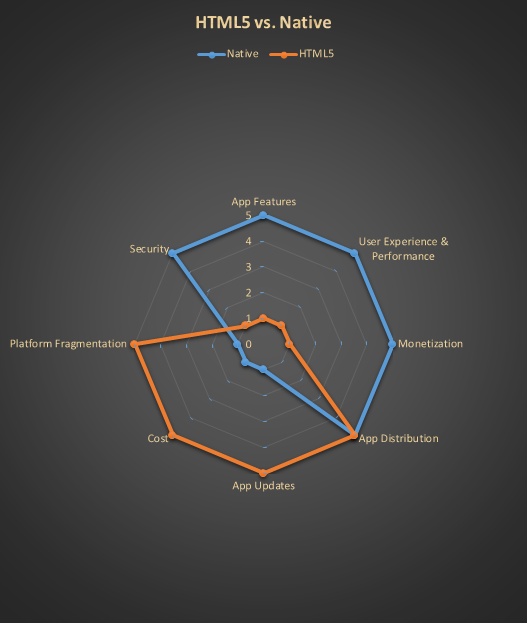
\includegraphics[width=1.0\textwidth]{hybrid_native_graph.png}
\caption{Slabiny a přednosti nativního a hybridního přístupu \cite{mobile_dev_nat_hybrid_graph}}
\label{fig:HybridNativeGraph}
\end{figure}